\section{Additionneurs quantiques de Draper}

Thomas G. Draper a proposé une méthode utilisant la QFT afin d'implémenter un additionneur quantique capable d'additionner la valeur binaire d'un nombre classique à celle d'un registre quantique \cite{draper2000additionquantumcomputer}. D'ailleurs, on peut l'adapter pour additionner la valeur binaire de deux registres quantiques \cite{draper2000additionquantumcomputer}. On présente les détails mathématiques ainsi que leur implémentation avec un circuit quantique.

\subsection{Additionneur $\Phi$ADD$_a$}
On montre dans cette section comment implémenter un additionneur quantique qui ajoute une valeur classique à un registre quantique. Soient $a$ et $b$ deux entiers binaires non-signés sur $n$ bits. On commence par encoder dans un registre quantique de $n$ qubits la valeur de $b$ pour obtenir $\ket*{b}$. Puis, on lui applique la QFT. Ensuite, sur chaque qubit $\ket*{\phi_j(b)}$, on applique une porte

\begin{equation}
    A_{j+1} = \prod_{k=1}^{j+1} R_k^{a_{j + 1 -k}} = \begin{bmatrix}
        1 & 0 \\
        0 & \prod_{k=1}^{j+1}e^{2\pi i a_{j+1-k}/2^k}
    \end{bmatrix} = 
    \begin{bmatrix}
        1 & 0 \\
        0 & e^{2\pi i \left(\frac{a_j}{2} + \frac{a_{j-1}}{4} + ... + \frac{a_0}{2^{j+1}}\right)}
    \end{bmatrix} =
    \begin{bmatrix}
        1 & 0 \\
        0 & e^{2\pi i a /2^{j+1}}
    \end{bmatrix}
\end{equation}

de telle sorte à obtenir 

\begin{equation*}
    A_{j+1}\ket*{\phi_j(b)}  = \frac{1}{\sqrt{2}} \left(\ket*{0} + e^{2\pi i \frac{b}{2^{j+1}}} e^{2\pi i \frac{a}{2^{j+1}}} \ket*{1}\right) = \frac{1}{\sqrt{2}} \left(\ket*{0} + e^{2\pi i \frac{(a+b)}{2^{j+1}}} \ket*{1}\right) = \ket*{\phi_j(a+b)}
\end{equation*}

Ainsi, après l'application des $A_{j+1}$ sur tous les qubits $\ket*{\phi_j(b)}$, on se retrouve globalement avec $\ket*{\phi(a+b)}$. On peut finalement appliquer la QFT inverse pour obtenir le résultat de l'addition. Il faut cependant faire attention à un potentiel débordement, car la somme de deux entiers à $n$ bits peut résulter en un entier à $n+1$ bits. Pour empêcher cela, on peut mettre $b$ dans un registre à $n+1$ qubits et mettre implicitement $a$ sur $n+1$ bits aussi (leur bit de poids fort étant forcément à 0) pour ensuite faire la même procédure. Au final,

\begin{equation}
    \Phi \text{ADD}_a \ket*{\phi(b)} = \ket*{\phi(a+b)}
\end{equation}

qu'on peut aisément implémenter avec un circuit quantique.

\begin{figure}[H]
    \centering
    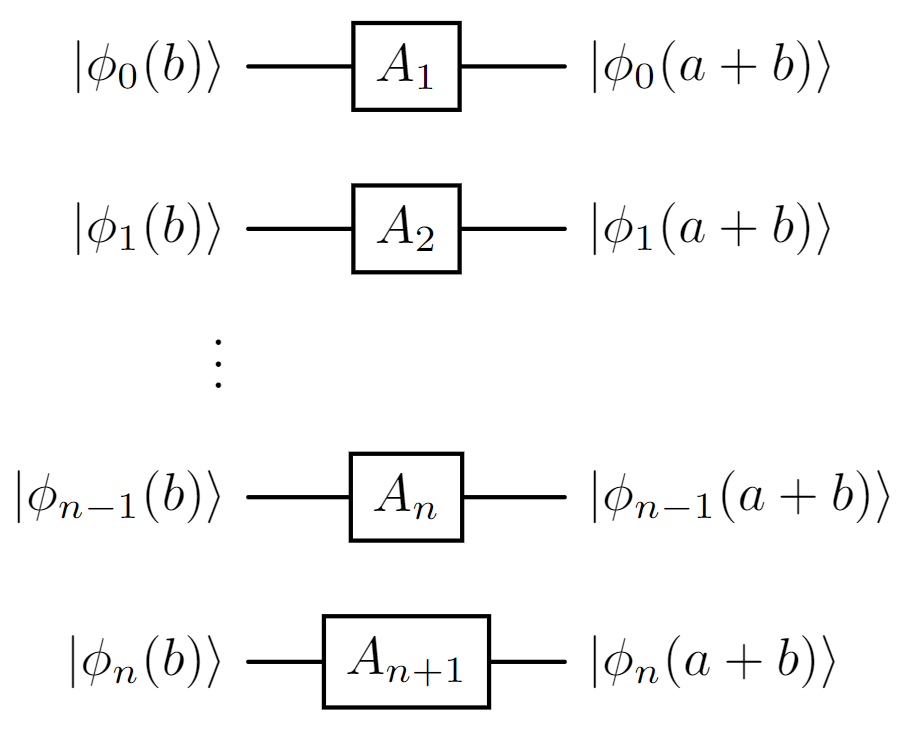
\includegraphics[scale=0.42]{images/phiadd.png} 
    \caption{Circuit pour $\Phi$ADD$_a$ avec la gestion du débordement}
\end{figure}

\subsection{Additionneur Q$\Phi$ADD}
On peut facilement adapter $\Phi$ADD$_a$ afin d'additionner deux entiers binaires non-signés $a$ et $b$ sur $n$ bits contenus chacun dans un registre quantique. Dans cette version, le résultat de l'addition se trouvera dans le registre contenant initialement $b$. On peut s'inspirer de la section précédente pour reproduire les $A_{j+1}$ en utilisant des opérations contrôlées par les qubits du registre contenant $a$. Effectivement, par (7), on voit que les portes $R_k$ sont appliquées ou non selon la valeur de $a_{j+1-k}$, puisque $R_k^1 = R_k$ et $R_k^0 = I$. Là aussi, on peut inclure la gestion du débordement avec un registre de $n+1$ qubits pour $b$. Dans ce cas, $a$ n'a pas aussi besoin d'être dans un registre de $n+1$ qubits, car comme $a$ est un entier sur $n$ bits, forcément $\ket*{a_n} = 0$ et il ne permettra d'appliquer aucune porte. En fait, on réalise le circuit comme si on avait deux registres à $n+1$ qubits, mais on omet $\ket*{a_n}$ et ce qu'il contrôle. En résumé, on a

\begin{equation}
    Q\Phi \text{ADD} (\ket*{a} \ket*{\phi(b)}) = \ket*{a} \ket*{\phi(a+b)}
\end{equation}

qu'on réalise facilement avec des portes $R_k$ contrôlées.

\begin{figure}[H]
    \centering
    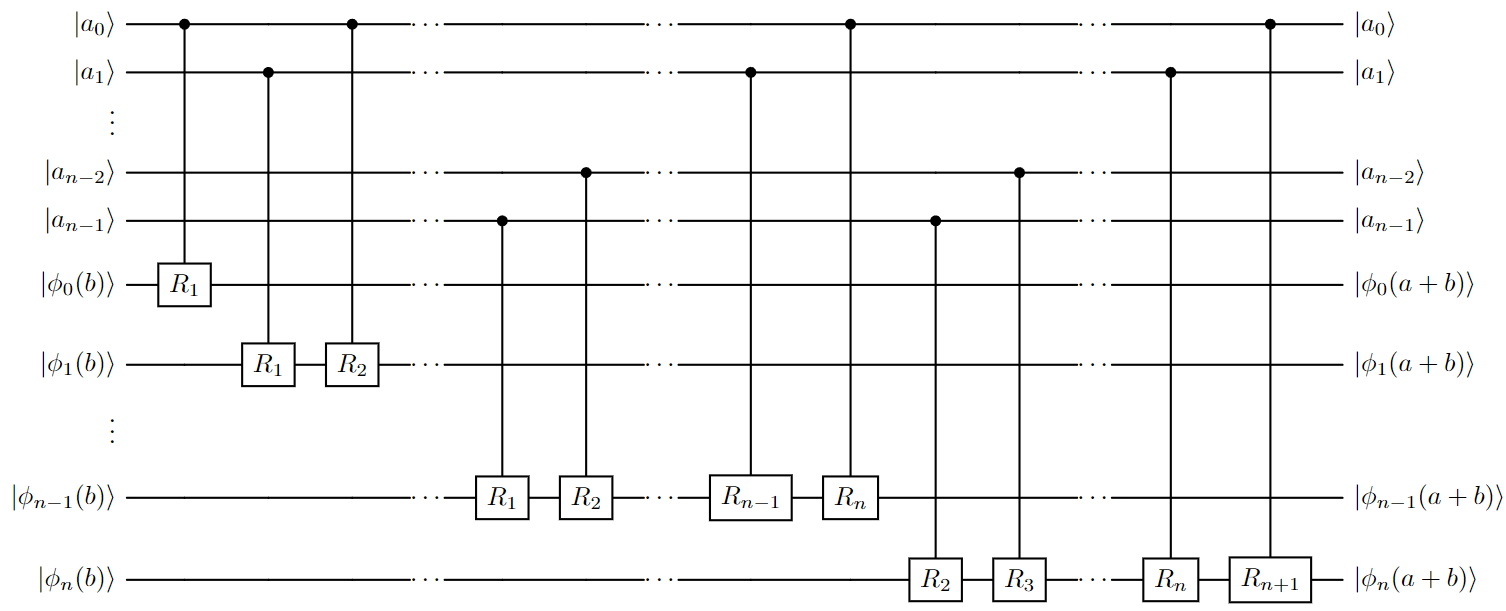
\includegraphics[scale=0.42]{images/qadd.png} 
    \caption{Circuit pour Q$\Phi$ADD avec la gestion du débordement}
\end{figure}

\subsection{$\Phi$ADD$_a$$^\dag$ et Q$\Phi$ADD$^\dag$}
Comme on s'en doute, $\Phi$ADD$_a$$^\dag$ et Q$\Phi$ADD$^\dag$ correspondent à des circuits qui effectuent une soustraction. 

\begin{equation*}
    A_{j+1}^\dag \ket*{\phi_j(b)}  = \frac{1}{\sqrt{2}} \left(\ket*{0} + e^{2\pi i \frac{b}{2^{j+1}}} e^{2\pi i \frac{-a}{2^{j+1}}} \ket*{1}\right) = \frac{1}{\sqrt{2}} \left(\ket*{0} + e^{2\pi i \frac{(b-a)}{2^{j+1}}} \ket*{1}\right) = \ket*{\phi_j(b-a)}
\end{equation*}

Cependant, $a$ et $b$ sont des entiers binaires non-signés et l'équation n'a du sens que si $b-a \geq 0$. Que se passe-t-il si $b-a < 0$?

Prenons comme exemple les valeurs $b = 1010_2$ et $a = 1100_2$ sur 4 bits. Alors, $b-a = -0010_2$, ce qui n'a pas de sens pour les nombres binaires non-signés. Dans ce cas, on veut trouver un entier positif équivalent à $b-a$.  Pour tous les entiers, il est trivial de dire que $(b-a) + a = b$. Donc, $(b-a) + 1100_2 = 1010_2$. Certes, la relation fonctionne avec $-0010_2$, mais aussi avec $1110_2$ qui est un entier positif. $1110_2$ fonctionne, car on travaille sur $4$ bits. Normalement, $1110_2 + 1100_2 = 11010_2$, mais on ne garde que les 4 premiers bits. Cela ramène le résultat à $11010_2 \text{ mod } 2^4 = 1010_2$ et la relation triviale tient. De ce fait, $-0010_2 \equiv 1110_2$. 

De manière générale, en écrivant $a$ et $b$ sur $n+1$ bits pour éviter un débordement, on trouve que $b-a = ((b-a) + 2^{n+1} ) \text{ mod } 2^{n+1}$ \cite{beauregard2003circuitshorsalgorithmusing}. Si $b \geq a$, alors forcément $((b-a) + 2^{n+1} ) \text{ mod } 2^{n+1} = b-a$. Sinon, $(b-a) + 2^{n+1}$ est forcément entre 0 et $2^{n+1}$, ce qui fait que  $((b-a) + 2^{n+1} ) \text{ mod } 2^{n+1} = (b-a) + 2^{n+1}$.

Ainsi, 

\begin{equation}
    \Phi \text{ADD}_a^\dag \ket*{\phi(b)} = 
    \begin{cases}
        \ket*{\phi(b-a)}, & \text{si \ } b \geq a \\
        \ket*{\phi((b-a) + 2^{n+1})}, & \text{sinon}
    \end{cases}
\end{equation}

\begin{equation}
    \text{Q}\Phi \text{ADD}^\dag (\ket*{a}\ket*{\phi(b)}) = 
    \begin{cases}
        \ket*{a} \ket*{\phi(b-a)}, & \text{si \ } b \geq a \\
        \ket*{a}\ket*{\phi((b-a) + 2^{n+1})}, & \text{sinon}
    \end{cases}
\end{equation}